\documentclass[11pt]{article}
\usepackage[margin=1in]{geometry}
\usepackage{amsmath,amssymb,amsthm,mathtools}
\usepackage{booktabs}
\usepackage{enumitem}
\usepackage{hyperref}
\usepackage{tikz}
\usetikzlibrary{arrows.meta,calc,positioning,fit}

\newcommand{\State}{\ensuremath{\mathsf{State}}}
\newcommand{\View}{\ensuremath{\mathsf{View}}}
\newcommand{\Worldline}{\ensuremath{\mathsf{Worldline}}}
\newcommand{\Strand}{\ensuremath{\mathsf{Strand}}}
\newcommand{\Braid}{\ensuremath{\mathsf{Braid}}}
\newcommand{\Conflict}{\ensuremath{\mathsf{Conflict}}}
\newcommand{\Witness}{\ensuremath{\mathsf{Witness}}}
\newcommand{\Lower}{\ensuremath{\mathsf{Lower}}}
\newcommand{\Canon}{\ensuremath{\mathsf{Canon}}}
\newcommand{\MJoin}{\ensuremath{\mathsf{Join}}}
\newcommand{\Lift}{\ensuremath{\mathsf{Lift}}}
\newcommand{\Cone}{\ensuremath{\mathsf{Cone}}}
\newcommand{\Merge}{\ensuremath{\mathsf{Merge}}}
\newcommand{\Proj}{\ensuremath{\pi}}
\newcommand{\Enriched}{\ensuremath{\mathcal{E}}}

\theoremstyle{definition}
\newtheorem{definition}{Definition}
\newtheorem{observation}{Observation}
\newtheorem{principle}{Principle}
\newtheorem{proposition}{Proposition}
\newtheorem{conjecture}{Conjecture}

\title{Merge Geometry and Theorem Spine\\[6pt]
\large What a Merge Really Is in a Causal / Optic Stack\\[3pt]
\normalsize 2026-04-09}
\author{}
\date{}

\begin{document}
\maketitle

\section{Purpose}

This note answers one question as directly as possible:

\begin{quote}
\emph{What is a merge, really, geometrically?}
\end{quote}

The answer proposed here is:

\begin{quote}
A merge is not fundamentally a text splice and not fundamentally a winner-pick.
Geometrically, a merge is the search for a lawful common extension of
concurrent causal rewrites relative to a shared precursor, together with a
witness of lawful lowering back to an observer-relative surface.
\end{quote}

Sometimes that common extension exists as an ordinary canonical state.
Sometimes it exists only in an enriched space that preserves explicit conflict.
Sometimes the system still needs policy to choose one public lowering.

\section{The Three Spaces}

The easiest way to avoid confusion is to distinguish three spaces.

\subsection{1. Lowered View Space}

This is the surface where ordinary tools often work:
\[
Y \in \View.
\]

Examples:
\begin{itemize}[leftmargin=2em]
\item a source file,
\item a JSON string,
\item a terminal rendering,
\item a debugger panel,
\item a filesystem materialization.
\end{itemize}

This space is useful, but often lossy.

\subsection{2. Canonical Causal Space}

This is the space of lawful causal states and worldlines:
\[
X \in \State.
\]

Here we still know:
\begin{itemize}[leftmargin=2em]
\item identity,
\item structure,
\item rewrite footprints,
\item causal order,
\item and the witnesses needed for lawful reassembly.
\end{itemize}

\subsection{3. Enriched Resolution Space}

Sometimes two branches have no single canonical join in $\State$, but we still
do not want to destroy either branch. So we admit a richer space:
\[
Z \in \Enriched.
\]

This space may contain:
\begin{itemize}[leftmargin=2em]
\item braid objects,
\item explicit conflict objects,
\item strand pairs,
\item residual / witness structure,
\item pending policy choices.
\end{itemize}

\begin{principle}[Where merge should happen]
If a system merges only in lowered view space, it will confuse projection
artifacts with real incompatibility. Merge should happen in the richest lawful
space available, and lowering should happen afterward with witness.
\end{principle}

\section{Branching and Future Cones}

Let $X_0$ be a shared precursor state. Two concurrent branches produce states
$X_A$ and $X_B$.

Each branch determines a set of lawful continuations:
\[
\Cone(X_A), \qquad \Cone(X_B).
\]

Geometrically, these are future cones of admissible continuation.

\begin{definition}[Canonical merge]
A \emph{canonical merge} of $X_A$ and $X_B$ is a state $M \in \State$ such that
\[
M \in \Cone(X_A) \cap \Cone(X_B)
\]
and $M$ lawfully preserves the committed meaning of both branches.
\end{definition}

This is the first important shift:

\begin{quote}
Merge is not ``blend these two text blobs.'' Merge is ``find a lawful common
future of these two causal branches.''
\end{quote}

\begin{figure}[h]
\centering
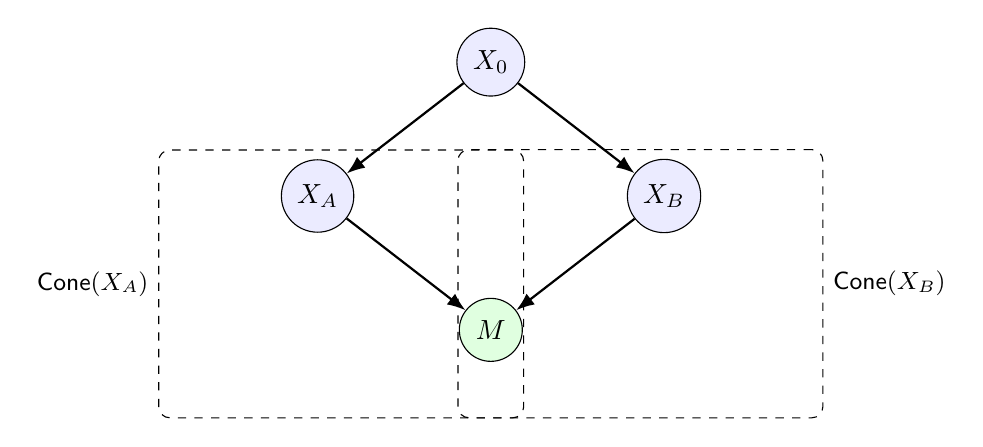
\begin{tikzpicture}[
  state/.style={draw, circle, minimum size=0.8cm, fill=blue!8},
  merge/.style={draw, circle, minimum size=0.8cm, fill=green!12},
  cone/.style={draw, rounded corners, dashed},
  arr/.style={-Latex, thick}
]
\node[state] (x0) at (0,4.2) {$X_0$};
\node[state] (xa) at (-2.2,2.5) {$X_A$};
\node[state] (xb) at (2.2,2.5) {$X_B$};
\node[merge] (m) at (0,0.8) {$M$};

\draw[arr] (x0) -- (xa);
\draw[arr] (x0) -- (xb);
\draw[arr] (xa) -- (m);
\draw[arr] (xb) -- (m);

\node[cone, fit={(xa) (-4.1,-0.2) (0.3,2.9)}, label=left:{\small $\Cone(X_A)$}] {};
\node[cone, fit={(xb) (-0.3,-0.2) (4.1,2.9)}, label=right:{\small $\Cone(X_B)$}] {};
\end{tikzpicture}
\caption{A canonical merge is a lawful common future of both branches.}
\end{figure}

\section{Why Text Merge Fails So Often}

Usually the system tries to merge in a projection:
\[
\Lower : \State \to \View.
\]

This is fine only when $\Lower$ preserves enough of the distinctions that make
the upstairs merge lawful. If it does not, then disjoint causal rewrites can
collapse onto overlapping view fragments.

\begin{observation}[Projection conflict]
A projection conflict occurs when:
\begin{enumerate}[leftmargin=2em]
\item there exists a lawful canonical merge upstairs in $\State$,
\item but the lowered views $\Lower(X_A)$ and $\Lower(X_B)$ do not admit an
  obvious merge downstairs in $\View$.
\end{enumerate}
\end{observation}

This is the precise version of ``merge conflicts happen because the merge is
happening through something lossy.''

\section{What a Genuine Conflict Is}

Not all conflicts are projection artifacts.

\begin{definition}[Genuine semantic conflict]
A genuine semantic conflict occurs when there is no lawful canonical common
extension in $\State$ that preserves the branch meanings simultaneously.
\end{definition}

Examples:
\begin{itemize}[leftmargin=2em]
\item two branches assign incompatible values to the same singleton slot,
\item two rewrites require mutually exclusive parentage or ownership,
\item two branches satisfy incompatible invariants.
\end{itemize}

\begin{observation}[Lifting is not magic]
Lifting cannot make contradictory semantics true at once. What lifting can do
is preserve both alternatives faithfully instead of destroying one under a
lossy merge policy.
\end{observation}

\section{Enriched Merge}

If the canonical intersection is empty in $\State$, the system can still admit
an enriched merge in $\Enriched$.

\begin{definition}[Enriched merge]
An \emph{enriched merge} of $X_A$ and $X_B$ is an object $Z \in \Enriched$ that
preserves both branches, together with explicit witness of why no immediate
canonical join exists.
\end{definition}

Typical enriched merge objects include:
\begin{itemize}[leftmargin=2em]
\item a braid over two strands,
\item a first-class conflict object,
\item a structured pair of competing witnesses,
\item a pending-governance object awaiting policy.
\end{itemize}

\begin{figure}[h]
\centering
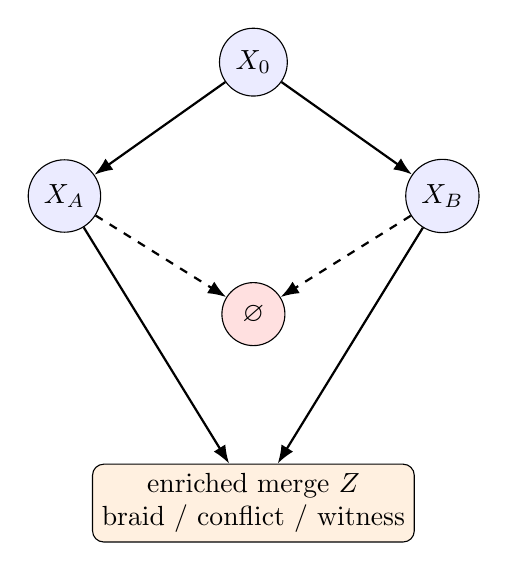
\begin{tikzpicture}[
  state/.style={draw, circle, minimum size=0.8cm, fill=blue!8},
  enrich/.style={draw, rounded corners, minimum width=2.9cm, minimum height=0.9cm, fill=orange!12, align=center},
  bad/.style={draw, circle, minimum size=0.8cm, fill=red!12},
  arr/.style={-Latex, thick}
]
\node[state] (x0) at (0,4.0) {$X_0$};
\node[state] (xa) at (-2.4,2.3) {$X_A$};
\node[state] (xb) at (2.4,2.3) {$X_B$};
\node[bad] (empty) at (0,0.8) {$\varnothing$};
\node[enrich] (z) at (0,-1.6) {enriched merge $Z$\\braid / conflict / witness};

\draw[arr] (x0) -- (xa);
\draw[arr] (x0) -- (xb);
\draw[arr,dashed] (xa) -- (empty);
\draw[arr,dashed] (xb) -- (empty);
\draw[arr] (xa) -- (z);
\draw[arr] (xb) -- (z);
\end{tikzpicture}
\caption{When no canonical join exists in $\State$, an enriched merge may still exist in $\Enriched$.}
\end{figure}

\section{What Is Lowering Back?}

After a canonical or enriched merge, the system often still needs a public
surface:
\[
\Lower_\omega : \State \text{ or } \Enriched \to \View.
\]

The subscript matters. Lowering requires witness:
\begin{itemize}[leftmargin=2em]
\item how identities serialize,
\item how focused regions reintegrate,
\item how ordering or formatting is chosen,
\item how conflict objects are rendered,
\item how redaction or observer policy is applied.
\end{itemize}

\begin{observation}[Lowering is not free]
Even if merge succeeds causally, lowering can still be ambiguous unless the
system carries enough witness and policy to produce a stable public form.
\end{observation}

\section{What a Merge Is in Optic Terms}

Suppose branch $A$ applies optic
\[
\Omega_A = (\pi_A,\phi_A,\rho_A,\omega_A,\sigma_A)
\]
and branch $B$ applies optic
\[
\Omega_B = (\pi_B,\phi_B,\rho_B,\omega_B,\sigma_B).
\]

Then merge asks:
\begin{enumerate}[leftmargin=2em]
\item do the footprints $\phi_A$ and $\phi_B$ commute?
\item if they commute, is there a lawful composed reintegration?
\item if they do not commute, what is the obstruction witness?
\item if no canonical composition exists, what enriched object preserves both
  optic results?
\item what witness lowers the result back into the intended observer surface?
\end{enumerate}

So in optic language:

\begin{quote}
Merge is the problem of composing concurrent optics over a shared precursor,
possibly by moving from canonical state space into an enriched space where the
obstruction itself becomes first-class.
\end{quote}

\section{The Geometric Core}

If you want one clean geometric statement, use this:

\begin{principle}[Merge as join-with-obstruction]
Geometrically, a merge is a search for a join of two branches in the space of
lawful continuations. If the join exists in canonical state space, merge
returns that join. If not, merge should return an enriched object that
preserves both branches and carries explicit witness of the obstruction.
\end{principle}

\section{Theorem Spine}

The following propositions and conjectures are the theorem-shaped heart of the
merge program.

\begin{proposition}[Projection-conflict proposition]
There exist branches $X_A, X_B \in \State$ and a projection
$\Lower : \State \to \View$ such that:
\begin{enumerate}[leftmargin=2em]
\item $X_A$ and $X_B$ admit a canonical merge $M \in \State$,
\item but $\Lower(X_A)$ and $\Lower(X_B)$ do not admit a canonical merge in
  the lowered view space.
\end{enumerate}
\end{proposition}

\begin{proposition}[Disjoint-footprint composition]
If two concurrent rewrites have lawfully disjoint footprints and compatible
reintegration witnesses, then they admit a canonical merge in $\State$.
\end{proposition}

\begin{proposition}[Semantic-obstruction proposition]
There exist concurrent rewrites for which no canonical merge exists in
$\State$, even though both rewrites are individually lawful from the shared
precursor.
\end{proposition}

\begin{proposition}[Enriched-merge proposition]
For some branch pairs with no canonical merge in $\State$, there exists an
enriched merge object $Z \in \Enriched$ preserving both branch meanings plus an
explicit obstruction witness.
\end{proposition}

\begin{proposition}[Lowering-with-witness proposition]
Lowering from $\State$ or $\Enriched$ into a public view is stable only
relative to sufficient witness and observer policy.
\end{proposition}

\begin{conjecture}[Conflict elimination by causal lifting]
For a large practical class of ordinary source-control conflicts, the apparent
conflict disappears when the merge is performed in a causal / structured space
that preserves identity, footprint, and witness.
\end{conjecture}

\begin{conjecture}[Conflict preservation by enrichment]
For a large practical class of genuine semantic conflicts, the correct outcome
is not forced resolution but enriched preservation, followed by later lowering
under explicit policy.
\end{conjecture}

\section{Research Questions}

These are the next useful questions if the theory is to become a real merge
engine:
\begin{enumerate}[leftmargin=2em]
\item What is the smallest witness required for stable lowering after a
  canonical merge?
\item What is the smallest witness required for enriched conflict rendering?
\item Which everyday Git conflicts are projection conflicts in disguise?
\item What is the best public noun for the enriched merge object:
  braid, conflict object, reconciliation object, or something else?
\item When does a policy-guided lowering count as canonical collapse, and when
  is it merely one observer among many?
\end{enumerate}

\section{One-Sentence Summary}

Geometrically, a merge is the search for a lawful common future of concurrent
causal branches, together with witness-bearing lowering back to a public view;
when no canonical common future exists, the right result is an enriched object
that preserves both branches and makes the obstruction explicit.

\end{document}
